\documentclass{article}

\usepackage{graphicx}

\usepackage{float}

\begin{document}

    \begin{titlepage}
        \centering

        {\Huge Data Cleaning, Automated Gathering and Analysis of European Parliament Voting Data\\}

        \vspace{1cm}

        {By \textbf{Franciszek Świderski}\\}

        \vspace{1cm}

        {B. Sc. International Politics and Government, Bocconi University\\}
        \vspace{1cm}
        {Under the supervision of\\}
        \vspace{1cm}

        {\textbf{Omiros Papaspilioupoulos}\\}

        \vspace{1cm}
        {Full Proffesor at Department of Decision Sciences, Bocconi University\\}
        \vspace{1cm}

        {For Institute for European Policymaking at Bocconi University\\}
        \vspace{1cm}
        {October 2024\\}

        \vspace{5cm} % Add some space between the title and author information


    \end{titlepage}


    \section{Introduction}

    The European Parliament voting data spanning the 6th to the 9th legislatures was inherited by the Institute for
    European Policy at Bocconi from the VoteWatch project, initially developed by Abdoul Noury and Simon Hix. To ensure
    the continuity and usability of this dataset, significant efforts were required in data cleaning, reformatting, and
    supplementation, followed by the automation of data gathering processes to facilitate ongoing maintenance. This
    dissertation details the systematic approach undertaken to clean and restructure the data, the challenges
    encountered, and the subsequent automation using the European Parliament's API, as well as the analysis conducted on
    using the data.

    \subsection{Dataset Structure and Initial Challenges}

    The dataset comprises three primary components:


    \begin{itemize}
        \item MepInfo: This dataset contains information on Members of the European Parliament (MEPs).
        \item Votes: This dataset records the votes cast by MEPs on specific pieces of legislation.
        \item Votings: This dataset describes the legislative items that were voted upon.
    \end{itemize}
    \begin{figure}[htb]
        \centering
        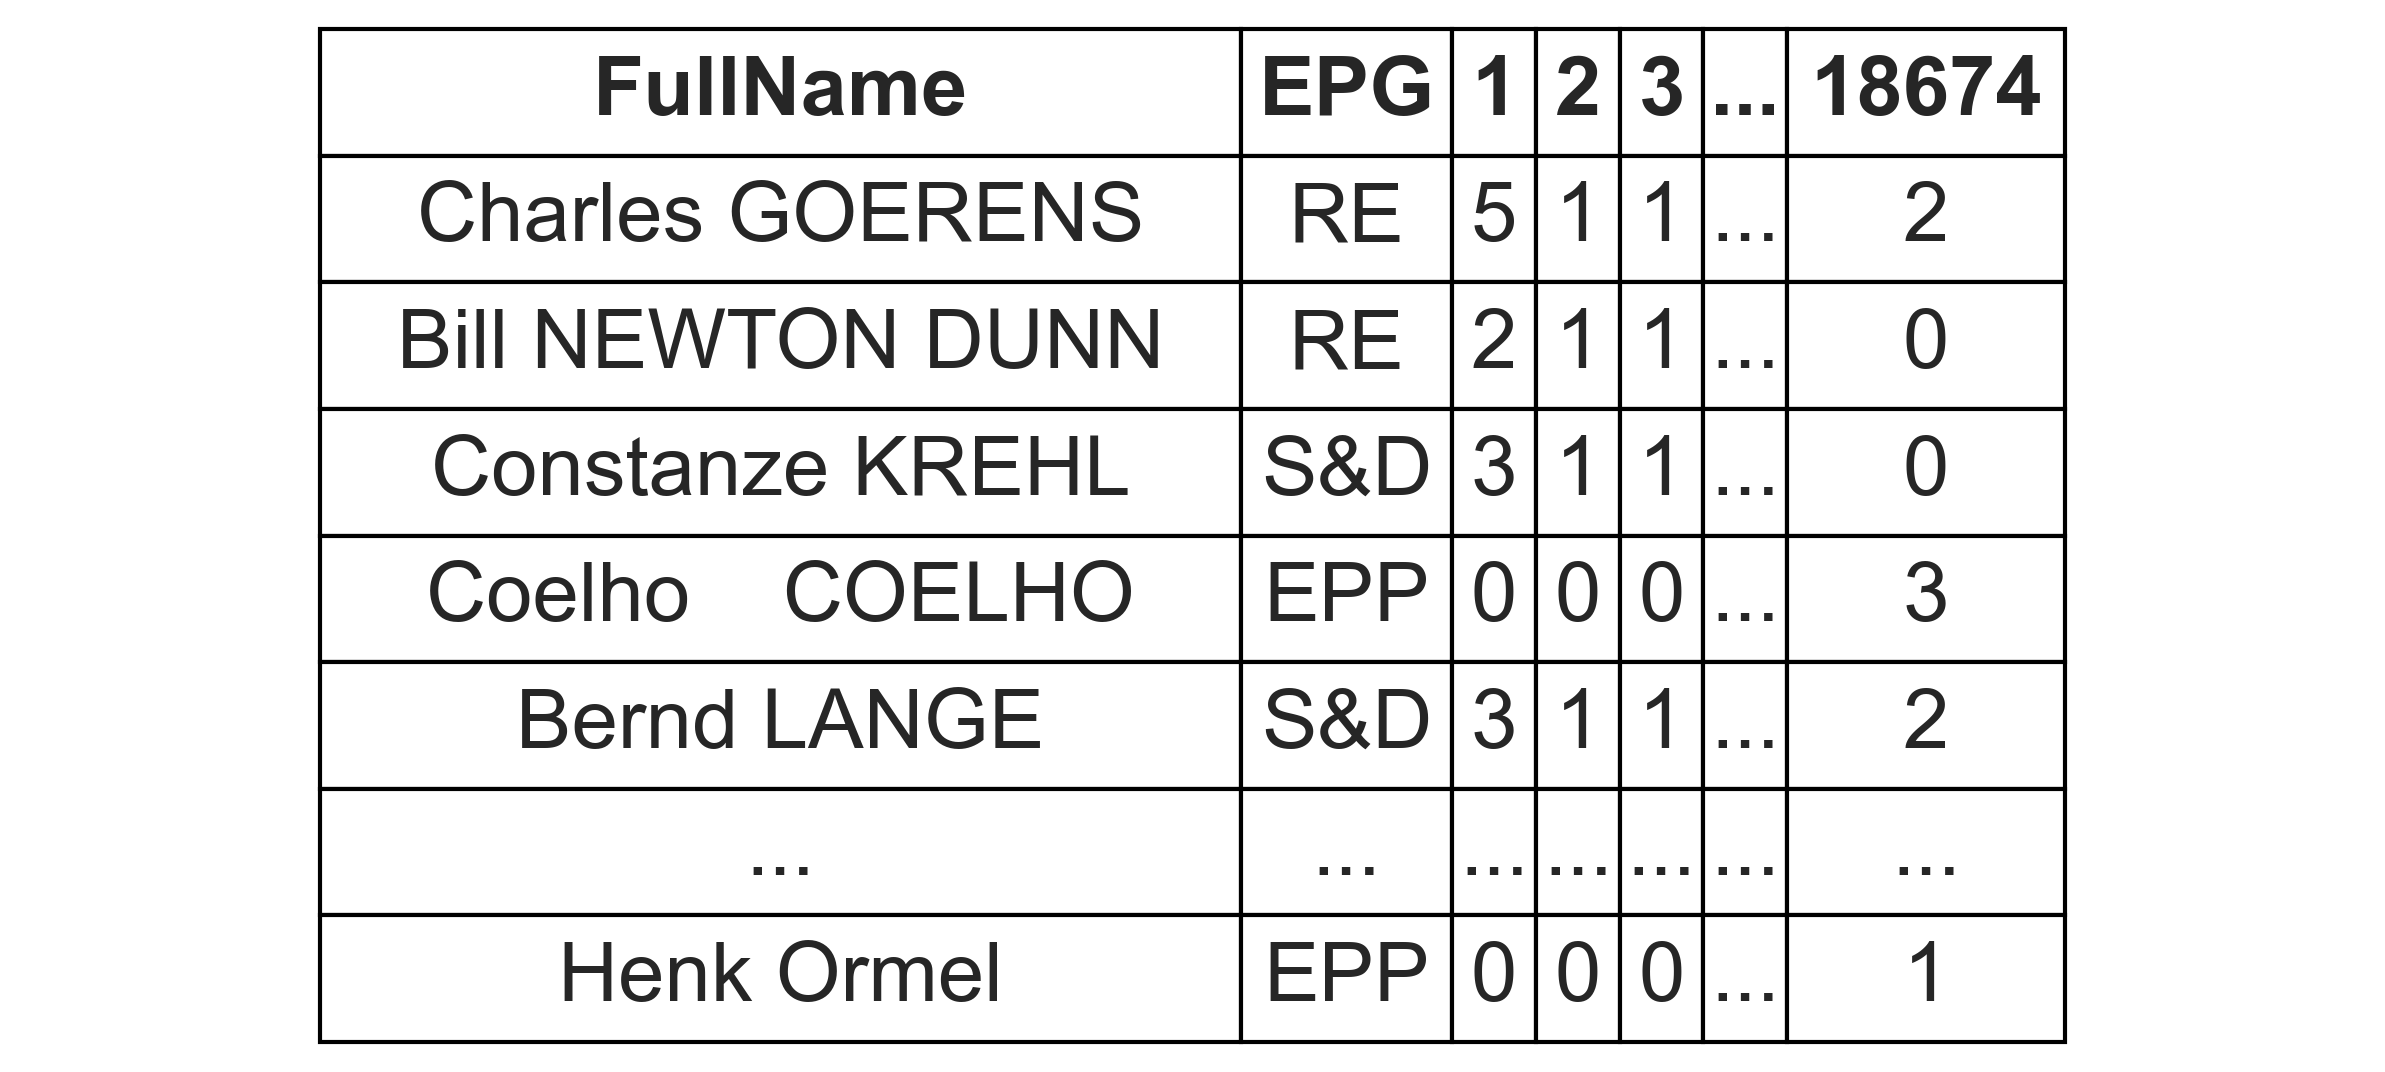
\includegraphics[width=1\textwidth]{Graphs/short_table9.png}
        \caption{Data from European Parliament 9 formatted for roll-call scaling}
        \label{fig:Structure table}
    \end{figure}

    The Votes dataset alone includes approximately 42,800 roll-calls, with 800-900 MEPs participating in each
    legislature, resulting in an estimated 40 million data points.
    \begin{figure}[htb]
        \centering
        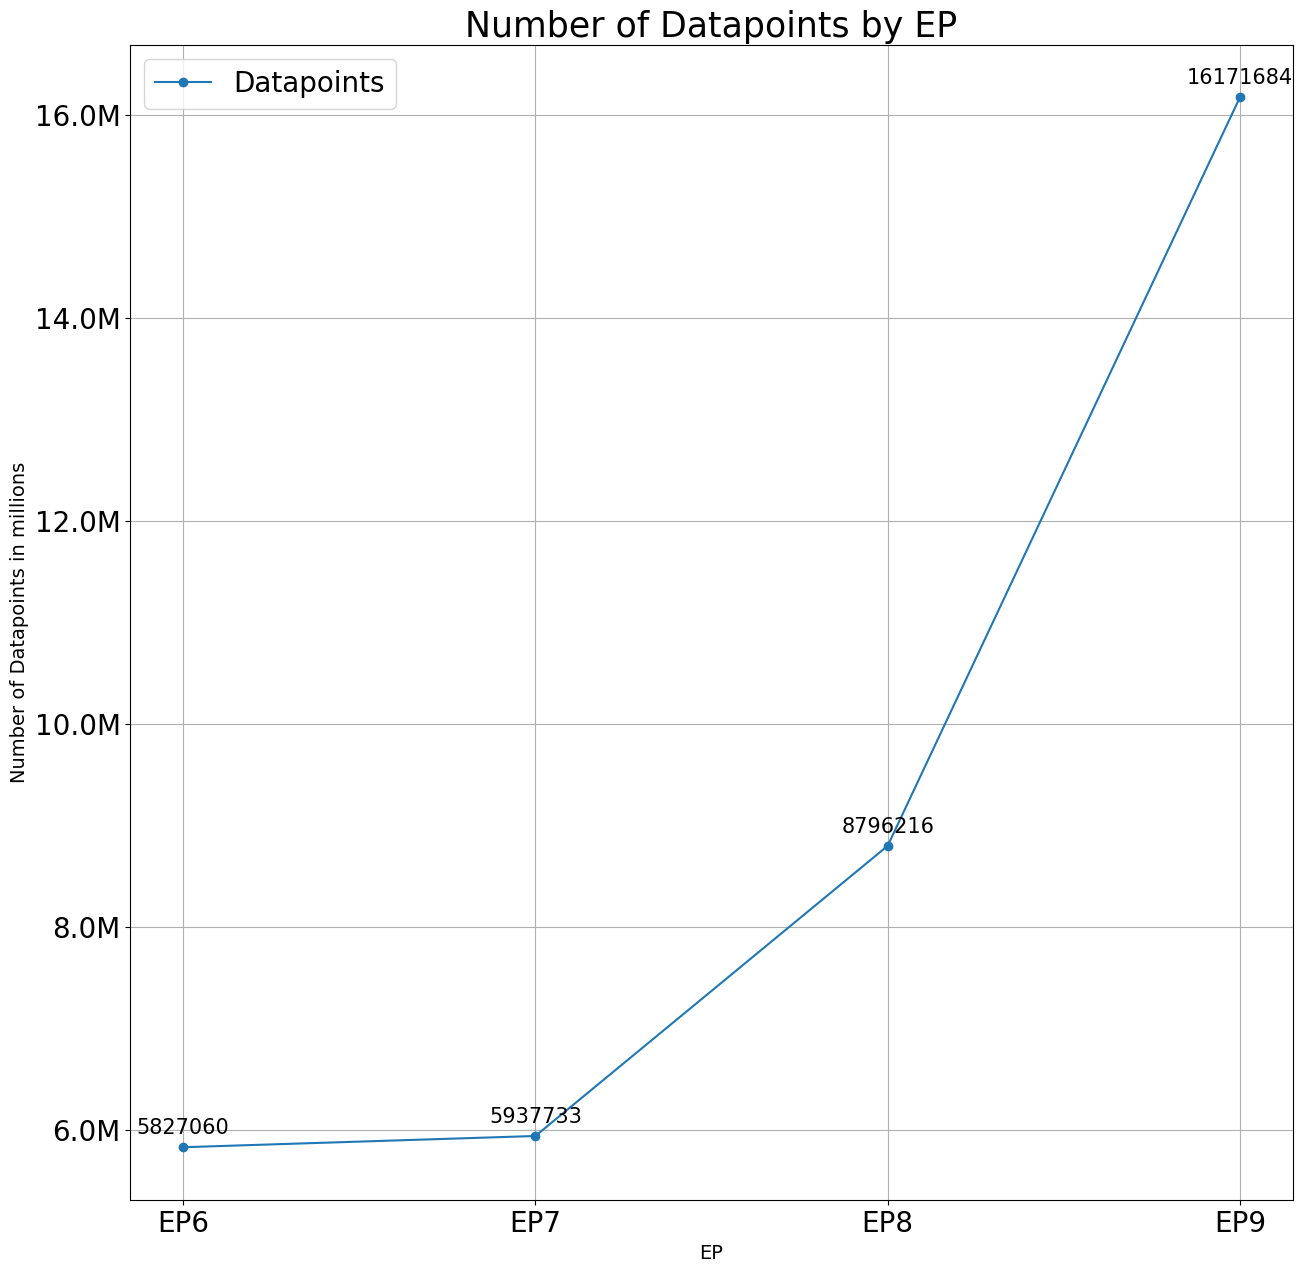
\includegraphics[width=0.8\textwidth]{Graphs/Datapoints.png}
        \caption{Number of datapoints by European Parliament (EP)}
        \label{fig:Datapoint graph}
    \end{figure}

    The size of the dataset makes for a serious practical challenge in terms of storage and processing, not to
    mention the problems with formatting and integrity of the dataset. Upon initial examination, several issues with the
    legacy data became apparent:

    \begin{itemize}
        \item Missing Variables: The MepInfo dataset lacked several critical variables, including gender and age.
        \item
        Inconsistencies and Missing Observations: Some variables such as Party affiliation and European Parliament Group
        (EPG) affiliation were either inconsistent or incomplete.
        \item
        Non-Standard MEP IDs in EP7: MEP IDs in the 7th Parliament did not conform to the standard European Parliament
        API format. Instead of unique identifiers, incrementing integers were used.
        \itemInconsistent Naming Conventions: MEP names and surnames were not consistent with those in the European
        Parliament API.
        \item
        Incorrect and Inconsistent Encoding of Missing Data: Missing data was inconsistently encoded, with symbols like
        - or . being used in place of null values.
        \item
        Inconsistent Datetime Formatting: Datetime values were formatted inconsistently across the dataset, making them
        difficult to import and process.
        \itemNon-Standard Encoding of Binary Categorical Variables: For example, the binary categorical variable "Vote,"
        which indicates whether a vote passed or not, was encoded as + and - instead of the standard 1/0 used elsewhere
        in the dataset.
    \end{itemize}
    Additionally, the dataset was stored in a long format tailored to the specific analytical requirements of the
    original VoteWatch team. While this structure was suited to their immediate needs, it posed challenges for long-term
    usability, warehousing, and broader analytical purposes.


    \section{Data Cleaning Process}

    \subsection{Supplementing and Correcting the MepInfo Dataset}


    The initial challenge involved supplementing and correcting the MepInfo dataset to fill in missing variables and
    rectify inconsistencies. The European Parliament's API played a crucial role in this process. An API (Application
    Programming Interface) is a set of defined rules and protocols that allows one software application to interact with
    another. In the context of scraping data, an API serves as an intermediary that lets users request and retrieve
    specific data from a website or service in a structured format, typically JSON or XML, without the need to manually
    scrape the HTML content of a webpage.
    Using an API for data scraping is often more efficient and reliable than traditional web scraping, as it provides
    direct access to the desired data, reducing the risk of encountering issues like changes in webpage structure or
    content restrictions. This API provides endpoints, such as `/meps`, which return JSON data containing basic MEP
    information, including a unique identifier (MepId). By utilizing this API, we were able to standardize the names and
    identifiers of MEPs across most legislatures by joining the tables by MepId.

    However, the 7th Parliament (EP7) presented a unique challenge. The MEP IDs in this legislature were not unique and
    were instead represented by incrementing integers. To address this issue, we employed the `fuzzywuzzy` Python
    package, which uses the Levenshtein distance algorithm to calculate the similarity between strings. This allowed for
    making an approximate match of full names from the original dataset to the `sortLabel` field in the API data,
    providing the correct MEP IDs. Manual verification and correction of edge cases were necessary to ensure accuracy.

    Despite these efforts, some data remained incomplete, particularly regarding MEPs who changed parties or EPGs during
    their tenure, as well as demographic data such as gender and birth dates. These gaps required further manual
    supplementation, which is discussed in detail in the Automation section.

    \subsection{Addressing Inconsistencies in the Votings Dataset}

    The Votings dataset required significant work to address encoding inconsistencies and improperly formatted datetime
    values. The first issue was relatively easy to reconcile using renaming dictionaries to replace inconsistent
    encodings in some variables.

    However, the latter issue proved particularly problematic due to the original data being gathered in Excel. Manual
    formatting likely led to inconsistent datetime values formatting. To standardize the format, manual correction of
    the dates was necessary before applying the Pandas `to datetime` function.

    This step ensured that the datetime values were correctly parsed and made the data suitable for further analysis.
    Once the initial cleaning was complete, a new challenge arose. In 2022, the original VoteWatch team altered their
    data gathering methodology. Consequently, data from Parliament 9, covering the period until 2022, was consistent
    with earlier practices. However, data collected from 2022 to March 2024 exhibited several discrepancies. The order
    of VoteIds had changed, some columns particularly those in the Votings dataset were missing, and special characters
    were corrupted due to encoding issues.
    To resolve these issues, we employed a multi-step approach. First, we used a dictionary to replace the corrupted
    characters systematically. Next, we reverse-engineered the missing Votings columns (such as finalVote, a binary
    variable of whether a vote is a last one in a section) from the available data. Despite the complexity of these
    tasks, they were necessary to restore the integrity and consistency of the dataset, ensuring that it could be
    seamlessly integrated with the existing data from earlier legislative periods.

    \subsection{Data Restructuring for Long-Term Usability}

    With the Votes and MepInfo datasets cleaned and supplemented, the next step was to restructure the data into a
    format suitable for long-term storage, analysis, and future updates. The data was initially stored in a long format,
    where each row represented an observation, and columns represented variables. To facilitate analysis, we separated
    the MepInfo and Votes datasets into distinct tables:
    \begin{itemize}
        \item MepInfo table contained all variables describing the MEPs, with `MepId` serving as the primary key.
        \item
        The Votes table used a composite primary key consisting of `MepId` and `VoteId`, a unique identifier for each
        voting event. This table also included a column encoding the MEPs' votes.
    \end{itemize}

    These tables were linked by primary keys, allowing for efficient querying and data retrieval. For example, using the
    `MepId`, one could easily retrieve all votes cast by a particular MEP, and by further referencing the `VoteId`,
    additional context from the Votings table could be added.

    To support the development of the European Parliament Vote Monitor website, the voting data was additionally
    exported in `.csv` format, organized by month and year. This format was chosen to optimize data storage and
    accessibility, ensuring that the data could be easily updated and queried. Additionally, for specialized analytical
    purposes, the Votes data was also retained in its original matrix format, now enhanced with the newly cleaned and
    supplemented variables.


    \section{Automation of Data Gathering}

    \subsection{Overview of the European Parliament API}

    With the historical data cleaned and restructured, the next phase of the project focused on automating the future
    data gathering process. Consistency and reliability were paramount in this process. The previous VoteWatch team
    relied on scraping XML files from the human-readable official minutes on the European Parliament's website, coupled
    with downloading MepInfo from the API. This approach was fraught with challenges, including the potential for
    inconsistencies in the scraped data, lack of unique identifiers, and the inherent unreliability of scraping
    human-readable content.

    To address these issues, we transitioned to using the European Parliament's open API, which provides direct access
    to structured data in a reliable and consistent manner. The API is publicly accessible, meaning no API key is
    required, and it allows users to specify parameters in the URI to retrieve data from various endpoints.

    \subsection{MepInfo Data Collection Automation}
    The `/meps` endpoint of the API, which provides a list of MEPs along with their unique identifiers, was the starting
    point for automating the MepInfo data collection. However, the data returned by this endpoint was not exhaustive. To
    gather more detailed information such as MEPs' gender, age, and political affiliations additional API calls were
    required to other endpoints within the `meps` group.

    For example, to retrieve data on MEPs' party memberships and affiliations with European Political Groups (EPGs) and
    National Parties, separate API calls were made specyfing the MepId . The resulting data was then filtered and joined
    with the MepInfo dataset to create a comprehensive record of each MEP s political affiliations and demographic
    information.

    One key challenge in this process was optimizing the API calls to minimize the load on the server. Each MEP required
    an individual API call to gather detailed data, which could result in approximately 850 GET requests per scraping
    session. To mitigate this, the metadata was included in the same call to avoid the need for additional requests.

    Another consideration was the use of non-human-readable IDs for certain values, such as the organization field,
    which required further API calls to retrieve the corresponding labels from the `corporate-bodies` endpoint. For
    example org/1537 was an identifier for GUE/NGL EU Political Group. These labels were essential for understanding the
    data and were subsequently joined with the MEPs' political affiliation data.

    \subsection{Votings Data Collection Automation}

    The `meetings` endpoint of the API was utilized to automate the collection of data on plenary sessions and the
    decisions made during these sessions. An initial API call returned a list of all plenary sessions that took place in
    a given year. This list was then filtered by month to identify the specific sessions relevant to the current data
    collection period.

    For each identified session, further API calls were made to retrieve detailed voting data, such as the votes cast by
    each individual member and all of the supplementary data that was previously found in the Votings database. This
    data was then merged with the previously gathered MepInfo and Votes data, ensuring that all relevant information was
    captured and linked across the collection.

    In order to automatically gather the data in the future, working with a Bocconi IT Department team, we created a
    cloud-based solution that is deployed and triggers every month, gathering and exporting the data to the .csv format,
    as well as to a relational SQL database.


    \section{Ideal points analysis}

    \subsection{Ideal Points Estimation workflow reproduction}
    The gathered data has proven invaluable for research into the ideological dimensions of the European Parliament. A
    key focus of this research has been the estimation of "ideal points" which represent the ideological positions of
    Members of the European Parliament (MEPs) based on their voting behavior. The starting point for this analysis was
    to replicate the results of earlier research by Simon Hix and Abdul Noury, who explored the dimensions of ideology
    within the European Parliament. To achieve this, we used WNOMINATE, a well-established software tool designed
    specifically for analyzing ideal points in legislative bodies. By applying WNOMINATE to the data from the Sixth Term
    of the European Parliament, we successfully recreated the ideological map that Hix and Noury originally produced.
    \begin{figure}[H]
        \centering
        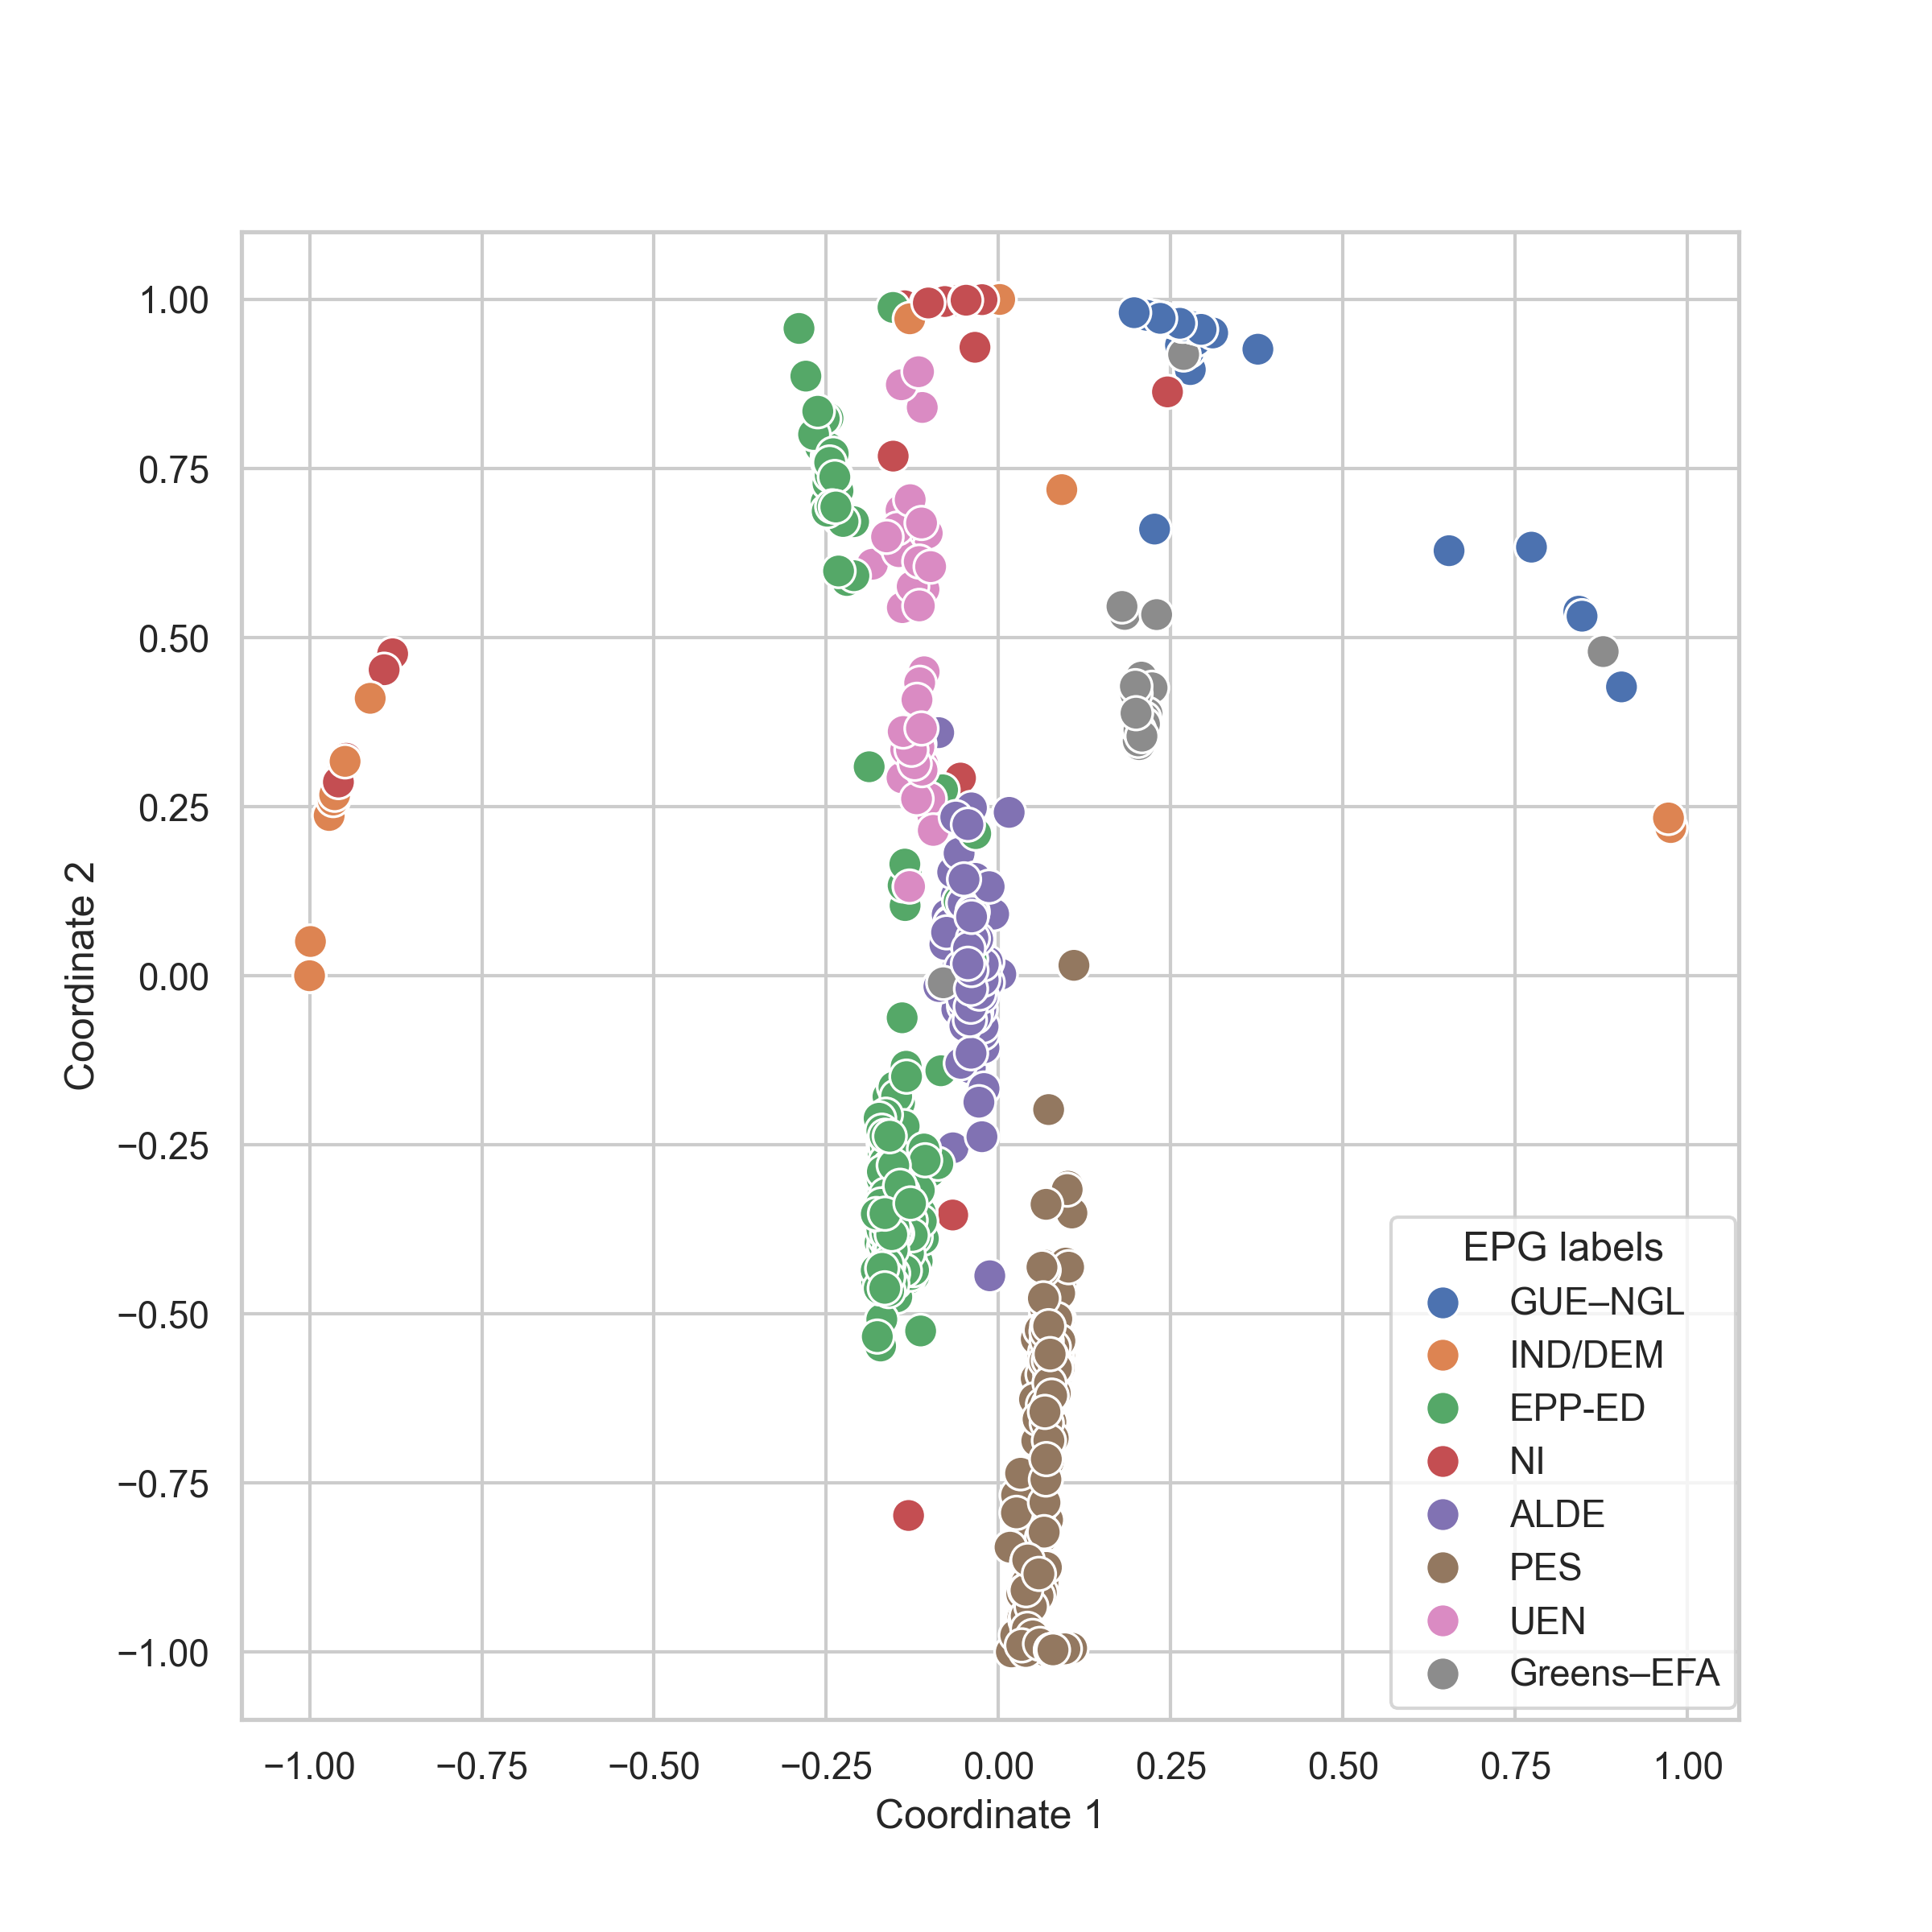
\includegraphics[width=1\textwidth]{Graphs/WNOMINATE2d.png}
        \caption{Recreation of Ideal Points Analysis in European Parliament 6 using WNOMINATE}
        \label{fig:WNOMINATE 6}
    \end{figure}

    The recreated graph revealed the expected dimensions of political ideology: a traditional left-right spectrum and a
    second dimension reflecting MEPs' stances on European integration, distinguishing between pro- and anti-European
    attitudes. These findings were consistent with the earlier work of Hix and Noury, confirming the validity of the
    dataset and the effectiveness of WNOMINATE in capturing these ideological divides.

    \subsection{Limitations of past methods and new solutions}
    As we extended the analysis to include later parliamentary terms, it became evident that WNOMINATE's performance was
    limited by the
    increasing size of the dataset. The software's computational demands grew significantly with the larger number of
    votes available in more recent parliaments, eventually rendering it impractical for further analysis.
    To overcome these limitations, we turned to a newer software tool, emIRT, developed in 2016 by Imai, Lo, and
    Olmsted.
    EmIRT is specifically designed to handle large datasets and is more efficient in estimating ideal points in complex
    spaces. By applying emIRT to the data from the later terms of the European Parliament, we was able to generate
    one-dimensional estimates of MEPs' ideological positions that accurately reflected the increased complexity of the
    dataset. The one-dimensionality, however, is the main drawback of the newer software, as the simplified
    dimensional space is traded off for computational efficiency. Nevertheless, the new, faster worklfow has enabled
    new methods and alleys of research - due to the flexibility of the software we was able to initialize the emIRT
    software with starting points calculated by WNOMINATE and seeing how it would impact the outcomes.

    \begin{figure}[H]
        \centering
        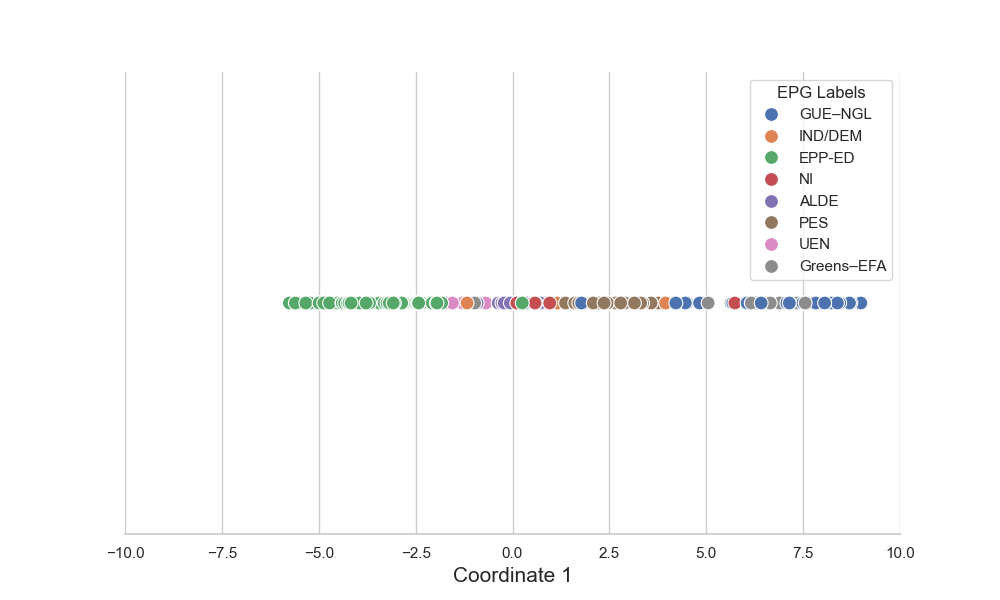
\includegraphics[width=1\textwidth]{Graphs/emIRT.png}
        \caption{One-dimensional ideal points estimation in European Parliament 6 using emIRT}
        \label{fig:emIRT}
    \end{figure}

    \subsection{Software research}
    In order to fully understand the software and its' results, and how one can tune the starting parameters we
    conducted
    an in-depth examination of the software's mechanics, gaining insight into its functional components and data
    processing algorithms. By delving into the underlying code and methodology, we developed a comprehensive
    understanding of how the software generates its starting points, processed the data and presents its' results.
    From this understanding came the ability to reverse-engineer and recreate some of the WNOMINATE solutions,
    particularly concerning the starting points of the ideal points estimation process.

    \subsection{Further development - Principal Component Analysis and Multi-Dimensional Ideal Points}
    With the workflow for estimating the ideal points established, we are expanding the research in other
    directions - namely, we are using methods of Primary Component Analysis (PCA) to enhance and compare with the
    results and starting points of the established software solutions. This work, while not yet ready, is showing
    promising results. Another area of interest that is being explored is multi-dimensional (3D,4D) ideal points
    estimations. Past research usually deems the high=dimensional estimations as less relevant, we believe that
    direction to be an interesting exploration.


    \section{Analysis of missing votes}

    The datasets not only include detailed information on the votes cast by Members of the European Parliament (MEPs)
    but also account for instances of missing votes, such as when an MEP is absent during a vote. This data,
    combined with the data on MEPs enriched with demographic information, is an interesting starting point towards
    identifying the structure behind the missingness, or why and which MEPs are absent during votes.

    \begin{figure}[htb]
        \centering
        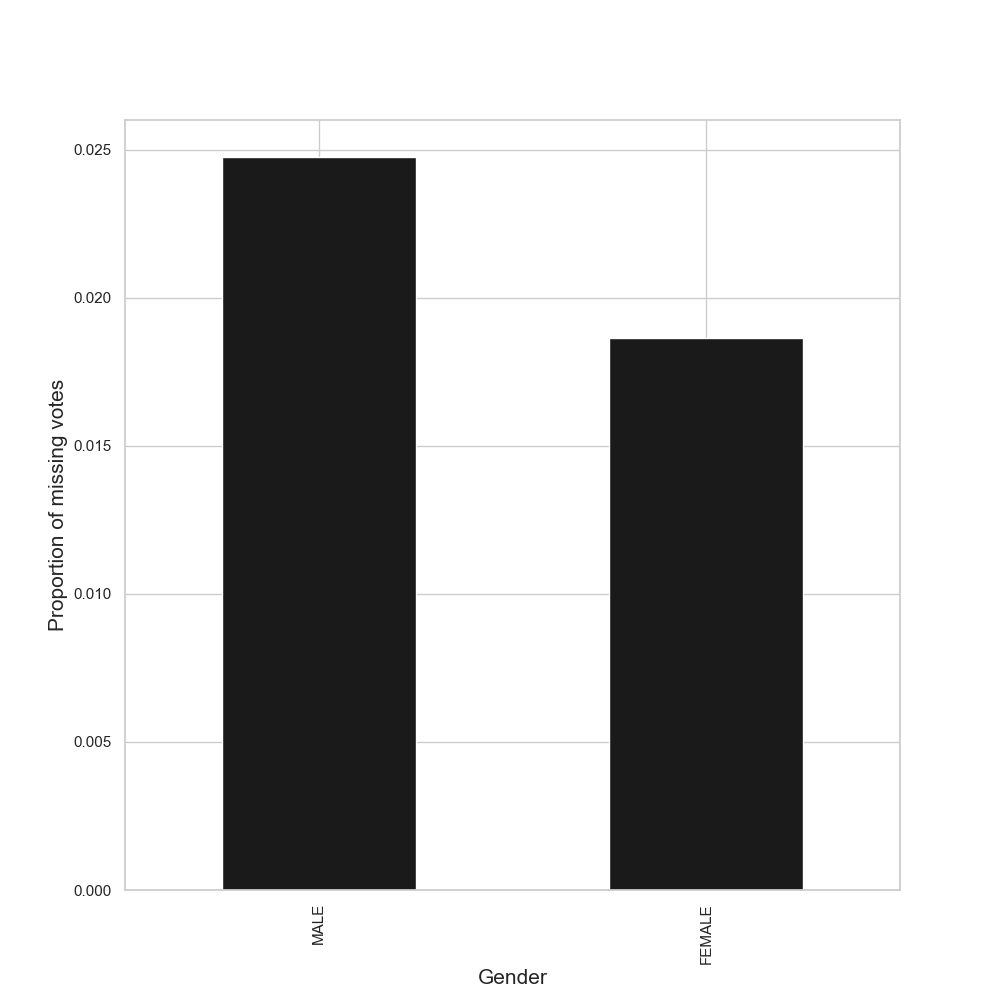
\includegraphics[width=\textwidth]{Graphs/genderreport.png}
        \caption
        {Proportion of missing votes by Gender in EP 9. Male MEPs are more likely to be absent than female ones.}
        \label{fig:gender}
    \end{figure}

    \subsection{Data visualization tool}
    While more rigorous analysis is required to establish causalty, descriptive statistics and visualizations are a
    good first step. To explore this aspect of the data, we developed an interactive data visualization
    tool that categorizes and sorts the proportion of absences by various factors, including country of origin, gender,
    and European Political Group (EPG) affiliation. This initial and crude implementation offers a basic yet
    informative view of
    absenteeism within the European Parliament, shedding light on how different demographic and political factors might
    correlate with voting attendance. As an example - male MEPs are consistently more absent than female MEPs (with
    exception of Parliament 8; See Figure~\ref{fig:gender}). Visualisation also gives an impression that eurosceptic
    or right-leaning parties tend to vote less often (See Figure~\ref{fig:proportions}).



    \begin{figure}[htb]
        \centering
        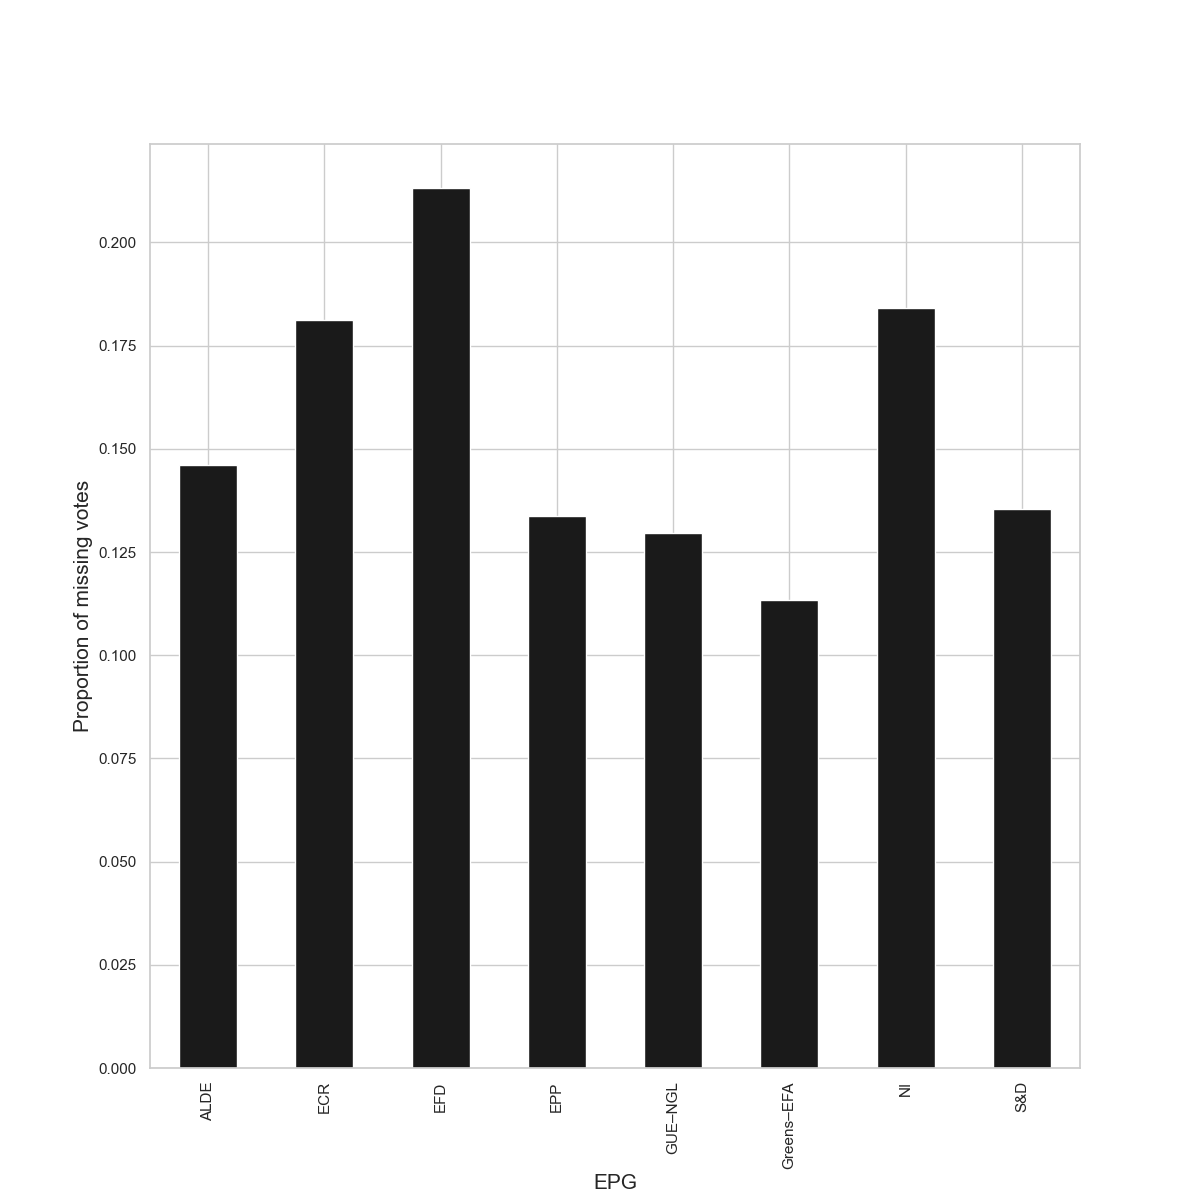
\includegraphics[width=\textwidth]{Graphs/proportions_report.png}
        \caption{Proportion of missing votes by EPG in EP 7}
        \label{fig:proportions}
    \end{figure}

    \subsection{Impact of ideology on missingness}
    In order to evaluate this claim, we decided on using the ideal points we obtained with the emIRT software. I
    checked the correlation of missingness and ideology, and while correlation of those two is indeed very low, it
    is slightly positive in most cases - meaning that the more right wing a MEP is, the more likely they are to miss
    a vote. Further research needs to be conducted to establish causality, but it is one of the many opportunities
    that the data presents before researchers.

    \subsection{Research development}
    Although this visualization and analysis is in its early stages, it has significant potential for further
    development.
    Enhancements could include more refined filtering options, additional variables for analysis, and integration with
    other datasets to provide deeper context. As part of the European Parliament Vote Monitor (EVPM) website, this tool
    could become a valuable feature for researchers, journalists, and the public, enabling them to explore patterns of
    MEP absenteeism in greater detail. By offering a clear and interactive way to analyse this data, the tool could help
    identify trends and raise important questions about the factors that influence MEPs' participation in legislative
    processes.


    \section{Conclusion}
    At this stage, the historical voting data from the European Parliament has been thoroughly cleaned, standardized,
    and is now ready for use by the Institute for European Policy and researchers. The efforts to address
    inconsistencies, fill in missing information, and standardize identifiers have made the dataset a more reliable
    resource for examining the dynamics of European legislative behavior.

    This work has ensured that the data is accessible and usable, providing a solid base for ongoing and future analyses.
    In addition to preparing the historical data, the implementation of an automated data gathering process ensures that
    the European Parliament Vote Monitor (EVPM) website will be continuously updated with the latest voting records and
    information on Members of the European Parliament (MEPs). Using the European Parliament’s API, this
    automated system will regularly collect and integrate new data, making it easier for researchers and policymakers to
    track developments in real time. This approach not only streamlines the process but also helps maintain the accuracy
    and relevance of the data available on the EVPM website.

    The project also establishes a consistent framework for analysing political ideology within the European Parliament.
    Initial analyses have successfully mapped traditional ideological dimensions using established methods like
    WNOMINATE and emIRT. Further research is ongoing, focusing on expanding these analyses into multi-dimensional spaces
    and exploring additional techniques like primary component analysis (PCA) and regression analysis. These efforts aim
    to provide a more detailed understanding of voting patterns and the factors that influence them, offering valuable
    insights into the ideological landscape of the European Parliament. The combination of cleaned data, automated
    updates, and thoughtful analysis positions this project as a valuable resource for future research and informed
    policymaking.

\end{document}